\documentclass[twoside]{book}

% Packages required by doxygen
\usepackage{fixltx2e}
\usepackage{calc}
\usepackage{doxygen}
\usepackage[export]{adjustbox} % also loads graphicx
\usepackage{graphicx}
\usepackage[utf8]{inputenc}
\usepackage{makeidx}
\usepackage{multicol}
\usepackage{multirow}
\PassOptionsToPackage{warn}{textcomp}
\usepackage{textcomp}
\usepackage[nointegrals]{wasysym}
\usepackage[table]{xcolor}

% Font selection
\usepackage[T1]{fontenc}
\usepackage[scaled=.90]{helvet}
\usepackage{courier}
\usepackage{amssymb}
\usepackage{sectsty}
\renewcommand{\familydefault}{\sfdefault}
\allsectionsfont{%
  \fontseries{bc}\selectfont%
  \color{darkgray}%
}
\renewcommand{\DoxyLabelFont}{%
  \fontseries{bc}\selectfont%
  \color{darkgray}%
}
\newcommand{\+}{\discretionary{\mbox{\scriptsize$\hookleftarrow$}}{}{}}

% Page & text layout
\usepackage{geometry}
\geometry{%
  a4paper,%
  top=2.5cm,%
  bottom=2.5cm,%
  left=2.5cm,%
  right=2.5cm%
}
\tolerance=750
\hfuzz=15pt
\hbadness=750
\setlength{\emergencystretch}{15pt}
\setlength{\parindent}{0cm}
\setlength{\parskip}{3ex plus 2ex minus 2ex}
\makeatletter
\renewcommand{\paragraph}{%
  \@startsection{paragraph}{4}{0ex}{-1.0ex}{1.0ex}{%
    \normalfont\normalsize\bfseries\SS@parafont%
  }%
}
\renewcommand{\subparagraph}{%
  \@startsection{subparagraph}{5}{0ex}{-1.0ex}{1.0ex}{%
    \normalfont\normalsize\bfseries\SS@subparafont%
  }%
}
\makeatother

% Headers & footers
\usepackage{fancyhdr}
\pagestyle{fancyplain}
\fancyhead[LE]{\fancyplain{}{\bfseries\thepage}}
\fancyhead[CE]{\fancyplain{}{}}
\fancyhead[RE]{\fancyplain{}{\bfseries\leftmark}}
\fancyhead[LO]{\fancyplain{}{\bfseries\rightmark}}
\fancyhead[CO]{\fancyplain{}{}}
\fancyhead[RO]{\fancyplain{}{\bfseries\thepage}}
\fancyfoot[LE]{\fancyplain{}{}}
\fancyfoot[CE]{\fancyplain{}{}}
\fancyfoot[RE]{\fancyplain{}{\bfseries\scriptsize Generated by Doxygen }}
\fancyfoot[LO]{\fancyplain{}{\bfseries\scriptsize Generated by Doxygen }}
\fancyfoot[CO]{\fancyplain{}{}}
\fancyfoot[RO]{\fancyplain{}{}}
\renewcommand{\footrulewidth}{0.4pt}
\renewcommand{\chaptermark}[1]{%
  \markboth{#1}{}%
}
\renewcommand{\sectionmark}[1]{%
  \markright{\thesection\ #1}%
}

% Indices & bibliography
\usepackage{natbib}
\usepackage[titles]{tocloft}
\setcounter{tocdepth}{3}
\setcounter{secnumdepth}{5}
\makeindex

% Hyperlinks (required, but should be loaded last)
\usepackage{ifpdf}
\ifpdf
  \usepackage[pdftex,pagebackref=true]{hyperref}
\else
  \usepackage[ps2pdf,pagebackref=true]{hyperref}
\fi
\hypersetup{%
  colorlinks=true,%
  linkcolor=blue,%
  citecolor=blue,%
  unicode%
}

% Custom commands
\newcommand{\clearemptydoublepage}{%
  \newpage{\pagestyle{empty}\cleardoublepage}%
}

\usepackage{caption}
\captionsetup{labelsep=space,justification=centering,font={bf},singlelinecheck=off,skip=4pt,position=top}

%===== C O N T E N T S =====

\begin{document}

% Titlepage & ToC
\hypersetup{pageanchor=false,
             bookmarksnumbered=true,
             pdfencoding=unicode
            }
\pagenumbering{alph}
\begin{titlepage}
\vspace*{7cm}
\begin{center}%
{\Large RL }\\
\vspace*{1cm}
{\large Generated by Doxygen 1.8.12}\\
\end{center}
\end{titlepage}
\clearemptydoublepage
\pagenumbering{roman}
\tableofcontents
\clearemptydoublepage
\pagenumbering{arabic}
\hypersetup{pageanchor=true}

%--- Begin generated contents ---
\chapter{Hierarchical Index}
\section{Class Hierarchy}
This inheritance list is sorted roughly, but not completely, alphabetically\+:\begin{DoxyCompactList}
\item \contentsline{section}{rl\+:\+:Action\+Experience\+Replay$<$ State\+Type, Action\+Type $>$}{\pageref{classrl_1_1_action_experience_replay}}{}
\item \contentsline{section}{rl\+:\+:Action\+Value\+Functor$<$ State\+Type, Action\+Type $>$}{\pageref{structrl_1_1_action_value_functor}}{}
\begin{DoxyCompactList}
\item \contentsline{section}{rl\+:\+:Continuous\+Action\+Value\+Functor$<$ State\+Type, Action\+Type $>$}{\pageref{structrl_1_1_continuous_action_value_functor}}{}
\begin{DoxyCompactList}
\item \contentsline{section}{rl\+:\+:Linear\+Action\+Value\+Functor$<$ State\+Type, Action\+Type $>$}{\pageref{classrl_1_1_linear_action_value_functor}}{}
\end{DoxyCompactList}
\item \contentsline{section}{rl\+:\+:Discrete\+Action\+Value\+Functor$<$ State\+Type, Action\+Type $>$}{\pageref{structrl_1_1_discrete_action_value_functor}}{}
\end{DoxyCompactList}
\item \contentsline{section}{rl\+:\+:Discrete\+Deterministic\+Policy$<$ State\+Type, Action\+Type $>$}{\pageref{classrl_1_1_discrete_deterministic_policy}}{}
\item \contentsline{section}{rl\+:\+:Discrete\+Epsilon\+Greedy\+Policy$<$ State\+Type, Action\+Type $>$}{\pageref{classrl_1_1_discrete_epsilon_greedy_policy}}{}
\item \contentsline{section}{rl\+:\+:Discrete\+Sarsa\+Lambda$<$ State\+Type, Action\+Type $>$}{\pageref{classrl_1_1_discrete_sarsa_lambda}}{}
\item \contentsline{section}{rl\+:\+:Discrete\+Td\+Lambda$<$ State\+Type, Action\+Type $>$}{\pageref{classrl_1_1_discrete_td_lambda}}{}
\item \contentsline{section}{rl\+:\+:Environment$<$ State\+Type, Action\+Type $>$}{\pageref{classrl_1_1_environment}}{}
\begin{DoxyCompactList}
\item \contentsline{section}{rl\+:\+:Continuous\+Environment$<$ State\+Type, Action\+Type $>$}{\pageref{classrl_1_1_continuous_environment}}{}
\item \contentsline{section}{rl\+:\+:Discrete\+Environment$<$ State\+Type, Action\+Type $>$}{\pageref{classrl_1_1_discrete_environment}}{}
\end{DoxyCompactList}
\item \contentsline{section}{rl\+:\+:Environment$<$ Grid\+State, Grid\+Action $>$}{\pageref{classrl_1_1_environment}}{}
\begin{DoxyCompactList}
\item \contentsline{section}{rl\+:\+:Discrete\+Environment$<$ Grid\+State, Grid\+Action $>$}{\pageref{classrl_1_1_discrete_environment}}{}
\begin{DoxyCompactList}
\item \contentsline{section}{rl\+:\+:Grid\+World}{\pageref{classrl_1_1_grid_world}}{}
\end{DoxyCompactList}
\end{DoxyCompactList}
\item \contentsline{section}{rl\+:\+:Environment$<$ Inverted\+Pendulum\+State, Inverted\+Pendulum\+Action $>$}{\pageref{classrl_1_1_environment}}{}
\begin{DoxyCompactList}
\item \contentsline{section}{rl\+:\+:Continuous\+Environment$<$ Inverted\+Pendulum\+State, Inverted\+Pendulum\+Action $>$}{\pageref{classrl_1_1_continuous_environment}}{}
\begin{DoxyCompactList}
\item \contentsline{section}{rl\+:\+:Inverted\+Pendulum}{\pageref{classrl_1_1_inverted_pendulum}}{}
\end{DoxyCompactList}
\end{DoxyCompactList}
\item \contentsline{section}{rl\+:\+:Grid\+Action}{\pageref{structrl_1_1_grid_action}}{}
\item \contentsline{section}{rl\+:\+:Grid\+State}{\pageref{structrl_1_1_grid_state}}{}
\item \contentsline{section}{rl\+:\+:Inverted\+Pendulum\+Action\+:\+:Hash}{\pageref{structrl_1_1_inverted_pendulum_action_1_1_hash}}{}
\item \contentsline{section}{rl\+:\+:Grid\+Action\+:\+:Hash}{\pageref{structrl_1_1_grid_action_1_1_hash}}{}
\item \contentsline{section}{rl\+:\+:Inverted\+Pendulum\+State\+:\+:Hash}{\pageref{structrl_1_1_inverted_pendulum_state_1_1_hash}}{}
\item \contentsline{section}{rl\+:\+:Grid\+State\+:\+:Hash}{\pageref{structrl_1_1_grid_state_1_1_hash}}{}
\item \contentsline{section}{rl\+:\+:Inverted\+Pendulum\+Action}{\pageref{structrl_1_1_inverted_pendulum_action}}{}
\item \contentsline{section}{rl\+:\+:Inverted\+Pendulum\+Params}{\pageref{structrl_1_1_inverted_pendulum_params}}{}
\item \contentsline{section}{rl\+:\+:Inverted\+Pendulum\+State}{\pageref{structrl_1_1_inverted_pendulum_state}}{}
\item \contentsline{section}{rl\+:\+:Modified\+Policy\+Iteration$<$ State\+Type, Action\+Type $>$}{\pageref{classrl_1_1_modified_policy_iteration}}{}
\item \contentsline{section}{rl\+:\+:State\+Experience\+Replay$<$ State\+Type $>$}{\pageref{classrl_1_1_state_experience_replay}}{}
\item \contentsline{section}{rl\+:\+:State\+Value\+Functor$<$ State\+Type $>$}{\pageref{structrl_1_1_state_value_functor}}{}
\begin{DoxyCompactList}
\item \contentsline{section}{rl\+:\+:Continuous\+State\+Value\+Functor$<$ State\+Type $>$}{\pageref{structrl_1_1_continuous_state_value_functor}}{}
\begin{DoxyCompactList}
\item \contentsline{section}{rl\+:\+:Linear\+State\+Value\+Functor$<$ State\+Type $>$}{\pageref{classrl_1_1_linear_state_value_functor}}{}
\end{DoxyCompactList}
\item \contentsline{section}{rl\+:\+:Discrete\+State\+Value\+Functor$<$ State\+Type $>$}{\pageref{structrl_1_1_discrete_state_value_functor}}{}
\end{DoxyCompactList}
\item \contentsline{section}{rl\+:\+:Td\+Lambda\+Params}{\pageref{structrl_1_1_td_lambda_params}}{}
\end{DoxyCompactList}

\chapter{Class Index}
\section{Class List}
Here are the classes, structs, unions and interfaces with brief descriptions\+:\begin{DoxyCompactList}
\item\contentsline{section}{\hyperlink{structrl_1_1_action_value_functor}{rl\+::\+Action\+Value\+Functor$<$ State\+Type, Action\+Type $>$} }{\pageref{structrl_1_1_action_value_functor}}{}
\item\contentsline{section}{\hyperlink{structrl_1_1_discrete_action_value_functor}{rl\+::\+Discrete\+Action\+Value\+Functor$<$ State\+Type, Action\+Type $>$} }{\pageref{structrl_1_1_discrete_action_value_functor}}{}
\item\contentsline{section}{\hyperlink{classrl_1_1_discrete_deterministic_policy}{rl\+::\+Discrete\+Deterministic\+Policy$<$ State\+Type, Action\+Type $>$} }{\pageref{classrl_1_1_discrete_deterministic_policy}}{}
\item\contentsline{section}{\hyperlink{classrl_1_1_discrete_environment}{rl\+::\+Discrete\+Environment$<$ State\+Type, Action\+Type $>$} }{\pageref{classrl_1_1_discrete_environment}}{}
\item\contentsline{section}{\hyperlink{classrl_1_1_discrete_epsilon_greedy_policy}{rl\+::\+Discrete\+Epsilon\+Greedy\+Policy$<$ State\+Type, Action\+Type $>$} }{\pageref{classrl_1_1_discrete_epsilon_greedy_policy}}{}
\item\contentsline{section}{\hyperlink{structrl_1_1_discrete_state_value_functor}{rl\+::\+Discrete\+State\+Value\+Functor$<$ State\+Type $>$} }{\pageref{structrl_1_1_discrete_state_value_functor}}{}
\item\contentsline{section}{\hyperlink{classrl_1_1_environment}{rl\+::\+Environment$<$ State\+Type, Action\+Type $>$} }{\pageref{classrl_1_1_environment}}{}
\item\contentsline{section}{\hyperlink{structrl_1_1_grid_action}{rl\+::\+Grid\+Action} }{\pageref{structrl_1_1_grid_action}}{}
\item\contentsline{section}{\hyperlink{structrl_1_1_grid_state}{rl\+::\+Grid\+State} }{\pageref{structrl_1_1_grid_state}}{}
\item\contentsline{section}{\hyperlink{classrl_1_1_grid_world}{rl\+::\+Grid\+World} }{\pageref{classrl_1_1_grid_world}}{}
\item\contentsline{section}{\hyperlink{structrl_1_1_grid_action_1_1_hash}{rl\+::\+Grid\+Action\+::\+Hash} }{\pageref{structrl_1_1_grid_action_1_1_hash}}{}
\item\contentsline{section}{\hyperlink{structrl_1_1_grid_state_1_1_hash}{rl\+::\+Grid\+State\+::\+Hash} }{\pageref{structrl_1_1_grid_state_1_1_hash}}{}
\item\contentsline{section}{\hyperlink{classrl_1_1_modified_policy_iteration}{rl\+::\+Modified\+Policy\+Iteration$<$ State\+Type, Action\+Type $>$} }{\pageref{classrl_1_1_modified_policy_iteration}}{}
\item\contentsline{section}{\hyperlink{structrl_1_1_state_value_functor}{rl\+::\+State\+Value\+Functor$<$ State\+Type $>$} }{\pageref{structrl_1_1_state_value_functor}}{}
\item\contentsline{section}{\hyperlink{classrl_1_1_td_lambda}{rl\+::\+Td\+Lambda$<$ State\+Type, Action\+Type $>$} }{\pageref{classrl_1_1_td_lambda}}{}
\item\contentsline{section}{\hyperlink{structrl_1_1_td_lambda_params}{rl\+::\+Td\+Lambda\+Params} }{\pageref{structrl_1_1_td_lambda_params}}{}
\end{DoxyCompactList}

\chapter{Class Documentation}
\hypertarget{structrl_1_1_action_value_functor}{}\section{rl\+:\+:Action\+Value\+Functor$<$ State\+Type, Action\+Type $>$ Struct Template Reference}
\label{structrl_1_1_action_value_functor}\index{rl\+::\+Action\+Value\+Functor$<$ State\+Type, Action\+Type $>$@{rl\+::\+Action\+Value\+Functor$<$ State\+Type, Action\+Type $>$}}
Inheritance diagram for rl\+:\+:Action\+Value\+Functor$<$ State\+Type, Action\+Type $>$\+:\begin{figure}[H]
\begin{center}
\leavevmode
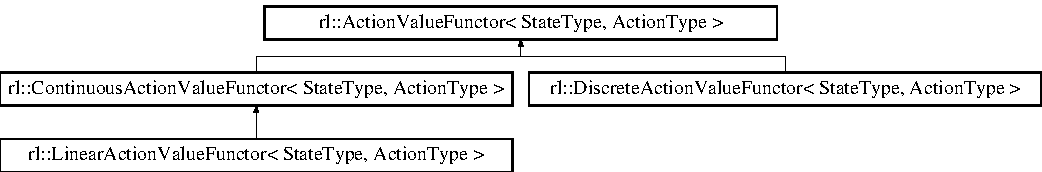
\includegraphics[height=2.000000cm]{structrl_1_1_action_value_functor}
\end{center}
\end{figure}
\subsection*{Public Member Functions}
\begin{DoxyCompactItemize}
\item 
\hypertarget{structrl_1_1_action_value_functor_af9cfc8284c860973783ddd4204b056b8}{}\label{structrl_1_1_action_value_functor_af9cfc8284c860973783ddd4204b056b8} 
virtual double {\bfseries operator()} (const State\+Type \&state, const Action\+Type \&action) const =0
\end{DoxyCompactItemize}


\subsection{Detailed Description}
\subsubsection*{template$<$typename State\+Type, typename Action\+Type$>$\newline
struct rl\+::\+Action\+Value\+Functor$<$ State\+Type, Action\+Type $>$}



Definition at line 49 of file action\+\_\+value\+\_\+functor.\+hpp.



The documentation for this struct was generated from the following file\+:\begin{DoxyCompactItemize}
\item 
/\+Users/davidfridovichkeil/\+Documents/\+Developer/rl/include/value/action\+\_\+value\+\_\+functor.\+hpp\end{DoxyCompactItemize}

\hypertarget{structrl_1_1_discrete_action_value_functor}{}\section{rl\+:\+:Discrete\+Action\+Value\+Functor$<$ State\+Type, Action\+Type $>$ Struct Template Reference}
\label{structrl_1_1_discrete_action_value_functor}\index{rl\+::\+Discrete\+Action\+Value\+Functor$<$ State\+Type, Action\+Type $>$@{rl\+::\+Discrete\+Action\+Value\+Functor$<$ State\+Type, Action\+Type $>$}}
Inheritance diagram for rl\+:\+:Discrete\+Action\+Value\+Functor$<$ State\+Type, Action\+Type $>$\+:\begin{figure}[H]
\begin{center}
\leavevmode
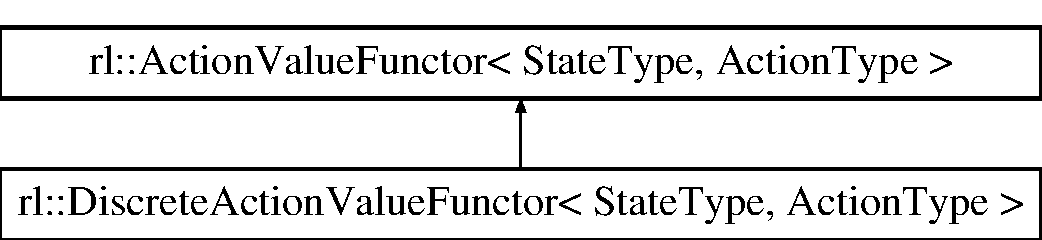
\includegraphics[height=2.000000cm]{structrl_1_1_discrete_action_value_functor}
\end{center}
\end{figure}
\subsection*{Public Member Functions}
\begin{DoxyCompactItemize}
\item 
\hypertarget{structrl_1_1_discrete_action_value_functor_a05b2e109cfcde8169b5cec710412cb54}{}\label{structrl_1_1_discrete_action_value_functor_a05b2e109cfcde8169b5cec710412cb54} 
void {\bfseries Set} (const State\+Type \&state, const Action\+Type \&action, double value)
\item 
\hypertarget{structrl_1_1_discrete_action_value_functor_a74c6f0ed5af23c049dafac2b7b02f8f6}{}\label{structrl_1_1_discrete_action_value_functor_a74c6f0ed5af23c049dafac2b7b02f8f6} 
double {\bfseries operator()} (const State\+Type \&state, const Action\+Type \&action) const
\end{DoxyCompactItemize}
\subsection*{Public Attributes}
\begin{DoxyCompactItemize}
\item 
\hypertarget{structrl_1_1_discrete_action_value_functor_aeb9044d42d523c3e068254555c84aa22}{}\label{structrl_1_1_discrete_action_value_functor_aeb9044d42d523c3e068254555c84aa22} 
std\+::unordered\+\_\+map$<$ State\+Type, std\+::unordered\+\_\+map$<$ Action\+Type, double, typename Action\+Type\+::\+Hash $>$, typename State\+Type\+::\+Hash $>$ {\bfseries value\+\_\+}
\end{DoxyCompactItemize}


\subsection{Detailed Description}
\subsubsection*{template$<$typename State\+Type, typename Action\+Type$>$\newline
struct rl\+::\+Discrete\+Action\+Value\+Functor$<$ State\+Type, Action\+Type $>$}



Definition at line 55 of file discrete\+\_\+action\+\_\+value\+\_\+functor.\+hpp.



The documentation for this struct was generated from the following file\+:\begin{DoxyCompactItemize}
\item 
/\+Users/davidfridovichkeil/\+Documents/\+Developer/rl/include/value/discrete\+\_\+action\+\_\+value\+\_\+functor.\+hpp\end{DoxyCompactItemize}

\hypertarget{classrl_1_1_discrete_deterministic_policy}{}\section{rl\+:\+:Discrete\+Deterministic\+Policy$<$ State\+Type, Action\+Type $>$ Class Template Reference}
\label{classrl_1_1_discrete_deterministic_policy}\index{rl\+::\+Discrete\+Deterministic\+Policy$<$ State\+Type, Action\+Type $>$@{rl\+::\+Discrete\+Deterministic\+Policy$<$ State\+Type, Action\+Type $>$}}
\subsection*{Public Member Functions}
\begin{DoxyCompactItemize}
\item 
\hypertarget{classrl_1_1_discrete_deterministic_policy_aa0502bdff3bbe4896d52b50e6fb682f3}{}\label{classrl_1_1_discrete_deterministic_policy_aa0502bdff3bbe4896d52b50e6fb682f3} 
void {\bfseries Set\+Randomly} (const \hyperlink{classrl_1_1_discrete_environment}{Discrete\+Environment}$<$ State\+Type, Action\+Type $>$ \&environment)
\item 
\hypertarget{classrl_1_1_discrete_deterministic_policy_ae1f5768f1189f650a37a280441a5a5f6}{}\label{classrl_1_1_discrete_deterministic_policy_ae1f5768f1189f650a37a280441a5a5f6} 
size\+\_\+t {\bfseries Set\+Greedily} (const typename \hyperlink{structrl_1_1_discrete_state_value}{Discrete\+State\+Value}$<$ State\+Type $>$\+::Const\+Ptr \&V, const \hyperlink{classrl_1_1_discrete_environment}{Discrete\+Environment}$<$ State\+Type, Action\+Type $>$ \&environment, double discount\+\_\+factor)
\item 
\hypertarget{classrl_1_1_discrete_deterministic_policy_a5361f9e8902b11c044953a44c39e0dbb}{}\label{classrl_1_1_discrete_deterministic_policy_a5361f9e8902b11c044953a44c39e0dbb} 
size\+\_\+t {\bfseries Set\+Greedily} (const typename \hyperlink{structrl_1_1_discrete_action_value}{Discrete\+Action\+Value}$<$ State\+Type, Action\+Type $>$\+::Const\+Ptr \&Q)
\item 
\hypertarget{classrl_1_1_discrete_deterministic_policy_aa464571566c0a6f97bb7e415fb78a491}{}\label{classrl_1_1_discrete_deterministic_policy_aa464571566c0a6f97bb7e415fb78a491} 
bool {\bfseries Act} (const State\+Type \&state, Action\+Type \&action) const
\end{DoxyCompactItemize}


\subsection{Detailed Description}
\subsubsection*{template$<$typename State\+Type, typename Action\+Type$>$\newline
class rl\+::\+Discrete\+Deterministic\+Policy$<$ State\+Type, Action\+Type $>$}



Definition at line 60 of file discrete\+\_\+deterministic\+\_\+policy.\+hpp.



The documentation for this class was generated from the following file\+:\begin{DoxyCompactItemize}
\item 
/\+Users/davidfridovichkeil/\+Documents/\+Developer/rl/include/policy/discrete\+\_\+deterministic\+\_\+policy.\+hpp\end{DoxyCompactItemize}

\hypertarget{classrl_1_1_discrete_environment}{}\section{rl\+:\+:Discrete\+Environment$<$ State\+Type, Action\+Type $>$ Class Template Reference}
\label{classrl_1_1_discrete_environment}\index{rl\+::\+Discrete\+Environment$<$ State\+Type, Action\+Type $>$@{rl\+::\+Discrete\+Environment$<$ State\+Type, Action\+Type $>$}}
Inheritance diagram for rl\+:\+:Discrete\+Environment$<$ State\+Type, Action\+Type $>$\+:\begin{figure}[H]
\begin{center}
\leavevmode
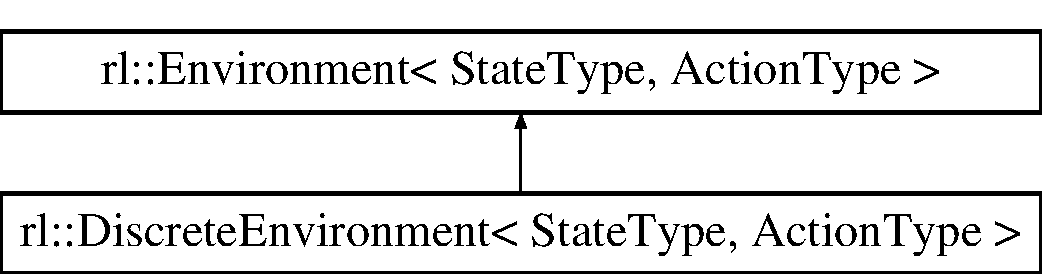
\includegraphics[height=2.000000cm]{classrl_1_1_discrete_environment}
\end{center}
\end{figure}
\subsection*{Public Member Functions}
\begin{DoxyCompactItemize}
\item 
\hypertarget{classrl_1_1_discrete_environment_a98f98b36d1a5148175e4307bba402f5e}{}\label{classrl_1_1_discrete_environment_a98f98b36d1a5148175e4307bba402f5e} 
virtual double {\bfseries Simulate} (State\+Type \&state, const Action\+Type \&action) const =0
\item 
\hypertarget{classrl_1_1_discrete_environment_a4e5f5e0425dc93dea82734b7327b22b8}{}\label{classrl_1_1_discrete_environment_a4e5f5e0425dc93dea82734b7327b22b8} 
virtual bool {\bfseries Is\+Valid} (const State\+Type \&state, const Action\+Type \&action) const =0
\item 
\hypertarget{classrl_1_1_discrete_environment_a7f41635b8c010b8a18a8661d0c2c0932}{}\label{classrl_1_1_discrete_environment_a7f41635b8c010b8a18a8661d0c2c0932} 
virtual bool {\bfseries Is\+Terminal} (const State\+Type \&state) const =0
\item 
\hypertarget{classrl_1_1_discrete_environment_a2cd36d24262dfc595574708f1118760f}{}\label{classrl_1_1_discrete_environment_a2cd36d24262dfc595574708f1118760f} 
virtual void {\bfseries States} (std\+::vector$<$ State\+Type $>$ \&states) const =0
\item 
\hypertarget{classrl_1_1_discrete_environment_a46561149e83e67db9e83d6d6169a9087}{}\label{classrl_1_1_discrete_environment_a46561149e83e67db9e83d6d6169a9087} 
virtual void {\bfseries Actions} (const State\+Type \&state, std\+::vector$<$ Action\+Type $>$ \&actions) const =0
\item 
\hypertarget{classrl_1_1_discrete_environment_ac9fc9c8f246e307509e6d041883ef89d}{}\label{classrl_1_1_discrete_environment_ac9fc9c8f246e307509e6d041883ef89d} 
virtual void {\bfseries Visualize} () const =0
\end{DoxyCompactItemize}


\subsection{Detailed Description}
\subsubsection*{template$<$typename State\+Type, typename Action\+Type$>$\newline
class rl\+::\+Discrete\+Environment$<$ State\+Type, Action\+Type $>$}



Definition at line 53 of file discrete\+\_\+environment.\+hpp.



The documentation for this class was generated from the following file\+:\begin{DoxyCompactItemize}
\item 
/\+Users/davidfridovichkeil/\+Documents/\+Developer/rl/include/environment/discrete\+\_\+environment.\+hpp\end{DoxyCompactItemize}

\hypertarget{classrl_1_1_discrete_epsilon_greedy_policy}{}\section{rl\+:\+:Discrete\+Epsilon\+Greedy\+Policy$<$ State\+Type, Action\+Type $>$ Class Template Reference}
\label{classrl_1_1_discrete_epsilon_greedy_policy}\index{rl\+::\+Discrete\+Epsilon\+Greedy\+Policy$<$ State\+Type, Action\+Type $>$@{rl\+::\+Discrete\+Epsilon\+Greedy\+Policy$<$ State\+Type, Action\+Type $>$}}
\subsection*{Public Member Functions}
\begin{DoxyCompactItemize}
\item 
\hypertarget{classrl_1_1_discrete_epsilon_greedy_policy_aa9d67bc59c160b060cb2fd4cc616fc66}{}\label{classrl_1_1_discrete_epsilon_greedy_policy_aa9d67bc59c160b060cb2fd4cc616fc66} 
{\bfseries Discrete\+Epsilon\+Greedy\+Policy} (double epsilon)
\item 
\hypertarget{classrl_1_1_discrete_epsilon_greedy_policy_a9559b1bfd5a8763e544a0aefd25f983d}{}\label{classrl_1_1_discrete_epsilon_greedy_policy_a9559b1bfd5a8763e544a0aefd25f983d} 
void {\bfseries Epsilon} () const
\item 
\hypertarget{classrl_1_1_discrete_epsilon_greedy_policy_aa9cef3d7f4c59af90a6f5edd8bcc8f2d}{}\label{classrl_1_1_discrete_epsilon_greedy_policy_aa9cef3d7f4c59af90a6f5edd8bcc8f2d} 
void {\bfseries Set\+Epsilon} (double epsilon)
\item 
\hypertarget{classrl_1_1_discrete_epsilon_greedy_policy_acc935a6aaee1988a35adcdcd1e5ed77c}{}\label{classrl_1_1_discrete_epsilon_greedy_policy_acc935a6aaee1988a35adcdcd1e5ed77c} 
void {\bfseries Set\+Randomly} (const \hyperlink{classrl_1_1_discrete_environment}{Discrete\+Environment}$<$ State\+Type, Action\+Type $>$ \&environment)
\item 
\hypertarget{classrl_1_1_discrete_epsilon_greedy_policy_a5dbcffbe61c91ad1a6ade8d3e51c572d}{}\label{classrl_1_1_discrete_epsilon_greedy_policy_a5dbcffbe61c91ad1a6ade8d3e51c572d} 
size\+\_\+t {\bfseries Set\+Greedily} (const typename \hyperlink{structrl_1_1_discrete_state_value}{Discrete\+State\+Value}$<$ State\+Type $>$\+::Const\+Ptr \&V, const \hyperlink{classrl_1_1_discrete_environment}{Discrete\+Environment}$<$ State\+Type, Action\+Type $>$ \&environment, double discount\+\_\+factor)
\item 
\hypertarget{classrl_1_1_discrete_epsilon_greedy_policy_a6d9264f4bf634832820ceae46436b028}{}\label{classrl_1_1_discrete_epsilon_greedy_policy_a6d9264f4bf634832820ceae46436b028} 
size\+\_\+t {\bfseries Set\+Greedily} (const typename \hyperlink{structrl_1_1_discrete_action_value}{Discrete\+Action\+Value}$<$ State\+Type, Action\+Type $>$\+::Const\+Ptr \&Q)
\item 
\hypertarget{classrl_1_1_discrete_epsilon_greedy_policy_a54e5c8fa9e5f473cfc1dd240c779728e}{}\label{classrl_1_1_discrete_epsilon_greedy_policy_a54e5c8fa9e5f473cfc1dd240c779728e} 
bool {\bfseries Act} (const \hyperlink{classrl_1_1_discrete_environment}{Discrete\+Environment}$<$ State\+Type, Action\+Type $>$ \&environment, const State\+Type \&state, Action\+Type \&action) const
\end{DoxyCompactItemize}


\subsection{Detailed Description}
\subsubsection*{template$<$typename State\+Type, typename Action\+Type$>$\newline
class rl\+::\+Discrete\+Epsilon\+Greedy\+Policy$<$ State\+Type, Action\+Type $>$}



Definition at line 60 of file discrete\+\_\+epsilon\+\_\+greedy\+\_\+policy.\+hpp.



The documentation for this class was generated from the following file\+:\begin{DoxyCompactItemize}
\item 
/\+Users/davidfridovichkeil/\+Documents/\+Developer/rl/include/policy/discrete\+\_\+epsilon\+\_\+greedy\+\_\+policy.\+hpp\end{DoxyCompactItemize}

\hypertarget{structrl_1_1_discrete_state_value_functor}{}\section{rl\+:\+:Discrete\+State\+Value\+Functor$<$ State\+Type $>$ Struct Template Reference}
\label{structrl_1_1_discrete_state_value_functor}\index{rl\+::\+Discrete\+State\+Value\+Functor$<$ State\+Type $>$@{rl\+::\+Discrete\+State\+Value\+Functor$<$ State\+Type $>$}}
Inheritance diagram for rl\+:\+:Discrete\+State\+Value\+Functor$<$ State\+Type $>$\+:\begin{figure}[H]
\begin{center}
\leavevmode
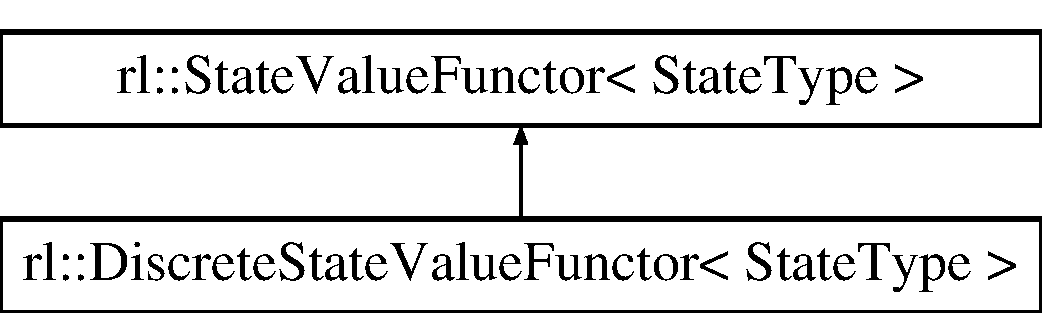
\includegraphics[height=2.000000cm]{structrl_1_1_discrete_state_value_functor}
\end{center}
\end{figure}
\subsection*{Public Member Functions}
\begin{DoxyCompactItemize}
\item 
\hypertarget{structrl_1_1_discrete_state_value_functor_a601e7ddfddf03e0bcef64ee855c89c80}{}\label{structrl_1_1_discrete_state_value_functor_a601e7ddfddf03e0bcef64ee855c89c80} 
void {\bfseries Set} (const State\+Type \&state, double value)
\item 
\hypertarget{structrl_1_1_discrete_state_value_functor_a63bf8449ed047b82326242424b8f1ef1}{}\label{structrl_1_1_discrete_state_value_functor_a63bf8449ed047b82326242424b8f1ef1} 
double {\bfseries operator()} (const State\+Type \&state) const
\item 
\hypertarget{structrl_1_1_discrete_state_value_functor_a6763e866eb6edad1a1b636dd75e15e99}{}\label{structrl_1_1_discrete_state_value_functor_a6763e866eb6edad1a1b636dd75e15e99} 
double \& {\bfseries operator\mbox{[}$\,$\mbox{]}} (const State\+Type \&state)
\item 
\hypertarget{structrl_1_1_discrete_state_value_functor_ac2c27101c79091445466bb4f3e5239c5}{}\label{structrl_1_1_discrete_state_value_functor_ac2c27101c79091445466bb4f3e5239c5} 
void {\bfseries Initialize} (const std\+::vector$<$ State\+Type $>$ \&states)
\end{DoxyCompactItemize}
\subsection*{Public Attributes}
\begin{DoxyCompactItemize}
\item 
\hypertarget{structrl_1_1_discrete_state_value_functor_a3467f778e304e14ddc44d271d41e0b6f}{}\label{structrl_1_1_discrete_state_value_functor_a3467f778e304e14ddc44d271d41e0b6f} 
std\+::unordered\+\_\+map$<$ State\+Type, double, typename State\+Type\+::\+Hash $>$ {\bfseries value\+\_\+}
\end{DoxyCompactItemize}


\subsection{Detailed Description}
\subsubsection*{template$<$typename State\+Type$>$\newline
struct rl\+::\+Discrete\+State\+Value\+Functor$<$ State\+Type $>$}



Definition at line 56 of file discrete\+\_\+state\+\_\+value\+\_\+functor.\+hpp.



The documentation for this struct was generated from the following file\+:\begin{DoxyCompactItemize}
\item 
/\+Users/davidfridovichkeil/\+Documents/\+Developer/rl/include/value/discrete\+\_\+state\+\_\+value\+\_\+functor.\+hpp\end{DoxyCompactItemize}

\hypertarget{classrl_1_1_environment}{}\section{rl\+:\+:Environment$<$ State\+Type, Action\+Type $>$ Class Template Reference}
\label{classrl_1_1_environment}\index{rl\+::\+Environment$<$ State\+Type, Action\+Type $>$@{rl\+::\+Environment$<$ State\+Type, Action\+Type $>$}}
Inheritance diagram for rl\+:\+:Environment$<$ State\+Type, Action\+Type $>$\+:\begin{figure}[H]
\begin{center}
\leavevmode
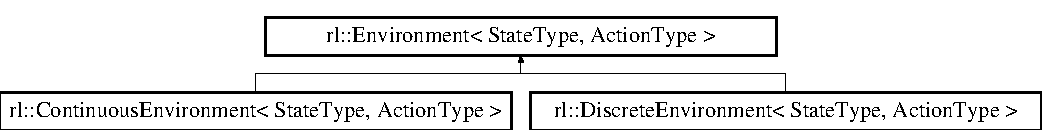
\includegraphics[height=2.000000cm]{classrl_1_1_environment}
\end{center}
\end{figure}
\subsection*{Public Member Functions}
\begin{DoxyCompactItemize}
\item 
\hypertarget{classrl_1_1_environment_ad97a592b7af8bb74859ebc82192feffe}{}\label{classrl_1_1_environment_ad97a592b7af8bb74859ebc82192feffe} 
virtual double {\bfseries Simulate} (State\+Type \&state, const Action\+Type \&action) const =0
\end{DoxyCompactItemize}


\subsection{Detailed Description}
\subsubsection*{template$<$typename State\+Type, typename Action\+Type$>$\newline
class rl\+::\+Environment$<$ State\+Type, Action\+Type $>$}



Definition at line 49 of file environment.\+hpp.



The documentation for this class was generated from the following file\+:\begin{DoxyCompactItemize}
\item 
/\+Users/davidfridovichkeil/\+Documents/\+Developer/rl/include/environment/environment.\+hpp\end{DoxyCompactItemize}

\hypertarget{structrl_1_1_grid_action}{}\section{rl\+:\+:Grid\+Action Struct Reference}
\label{structrl_1_1_grid_action}\index{rl\+::\+Grid\+Action@{rl\+::\+Grid\+Action}}
\subsection*{Public Types}
\begin{DoxyCompactItemize}
\item 
\hypertarget{structrl_1_1_grid_action_ab3b4b1b32a2a67afaf9c88bbe0527bb4}{}\label{structrl_1_1_grid_action_ab3b4b1b32a2a67afaf9c88bbe0527bb4} 
enum {\bfseries Direction} \{ {\bfseries UP}, 
{\bfseries D\+O\+WN}, 
{\bfseries L\+E\+FT}, 
{\bfseries R\+I\+G\+HT}
 \}
\end{DoxyCompactItemize}
\subsection*{Public Member Functions}
\begin{DoxyCompactItemize}
\item 
\hypertarget{structrl_1_1_grid_action_a993b14ba6d901d7174fe858ae558ef86}{}\label{structrl_1_1_grid_action_a993b14ba6d901d7174fe858ae558ef86} 
bool {\bfseries operator==} (const \hyperlink{structrl_1_1_grid_action}{Grid\+Action} \&rhs) const
\item 
\hypertarget{structrl_1_1_grid_action_a6ab02d4c6b0a70a83a8314429a33a176}{}\label{structrl_1_1_grid_action_a6ab02d4c6b0a70a83a8314429a33a176} 
bool {\bfseries operator==} (Grid\+Action\+::\+Direction rhs) const
\end{DoxyCompactItemize}
\subsection*{Public Attributes}
\begin{DoxyCompactItemize}
\item 
\hypertarget{structrl_1_1_grid_action_a064e3e1e58eef9d718cd0cadae0318b8}{}\label{structrl_1_1_grid_action_a064e3e1e58eef9d718cd0cadae0318b8} 
Direction {\bfseries direction\+\_\+}
\end{DoxyCompactItemize}


\subsection{Detailed Description}


Definition at line 50 of file grid\+\_\+action.\+hpp.



The documentation for this struct was generated from the following files\+:\begin{DoxyCompactItemize}
\item 
/\+Users/davidfridovichkeil/\+Documents/\+Developer/rl/include/environment/grid\+\_\+action.\+hpp\item 
/\+Users/davidfridovichkeil/\+Documents/\+Developer/rl/src/environment/grid\+\_\+action.\+cpp\end{DoxyCompactItemize}

\hypertarget{structrl_1_1_grid_state}{}\section{rl\+:\+:Grid\+State Struct Reference}
\label{structrl_1_1_grid_state}\index{rl\+::\+Grid\+State@{rl\+::\+Grid\+State}}
\subsection*{Public Member Functions}
\begin{DoxyCompactItemize}
\item 
\hypertarget{structrl_1_1_grid_state_a7aee8d309c9081f8b9f28d09eed9cc8d}{}\label{structrl_1_1_grid_state_a7aee8d309c9081f8b9f28d09eed9cc8d} 
{\bfseries Grid\+State} (size\+\_\+t ii, size\+\_\+t jj)
\item 
\hypertarget{structrl_1_1_grid_state_af911883b99f50f7169c808e7b72b04c9}{}\label{structrl_1_1_grid_state_af911883b99f50f7169c808e7b72b04c9} 
bool {\bfseries operator==} (const \hyperlink{structrl_1_1_grid_state}{Grid\+State} \&rhs)
\item 
\hypertarget{structrl_1_1_grid_state_a3a68e2226d51a3b1a5aa763873bb9e47}{}\label{structrl_1_1_grid_state_a3a68e2226d51a3b1a5aa763873bb9e47} 
bool {\bfseries operator!=} (const \hyperlink{structrl_1_1_grid_state}{Grid\+State} \&rhs)
\end{DoxyCompactItemize}
\subsection*{Public Attributes}
\begin{DoxyCompactItemize}
\item 
\hypertarget{structrl_1_1_grid_state_a91bf4c50c85c2980c6213c72ec468691}{}\label{structrl_1_1_grid_state_a91bf4c50c85c2980c6213c72ec468691} 
size\+\_\+t {\bfseries ii\+\_\+}
\item 
\hypertarget{structrl_1_1_grid_state_aa53f8a955bb8507589d0c023c5e3f958}{}\label{structrl_1_1_grid_state_aa53f8a955bb8507589d0c023c5e3f958} 
size\+\_\+t {\bfseries jj\+\_\+}
\end{DoxyCompactItemize}


\subsection{Detailed Description}


Definition at line 50 of file grid\+\_\+state.\+hpp.



The documentation for this struct was generated from the following file\+:\begin{DoxyCompactItemize}
\item 
/\+Users/davidfridovichkeil/\+Documents/\+Developer/rl/include/environment/grid\+\_\+state.\+hpp\end{DoxyCompactItemize}

\hypertarget{classrl_1_1_grid_world}{}\section{rl\+:\+:Grid\+World Class Reference}
\label{classrl_1_1_grid_world}\index{rl\+::\+Grid\+World@{rl\+::\+Grid\+World}}
Inheritance diagram for rl\+:\+:Grid\+World\+:\begin{figure}[H]
\begin{center}
\leavevmode
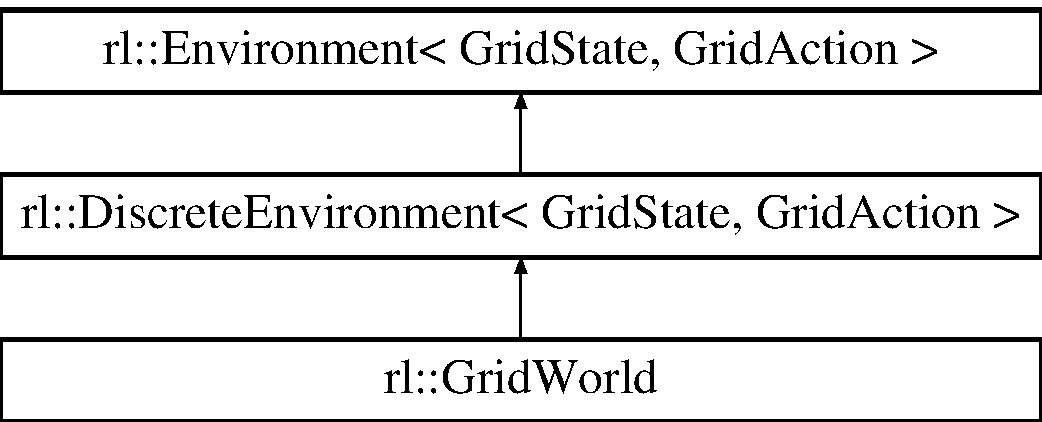
\includegraphics[height=2.000000cm]{classrl_1_1_grid_world}
\end{center}
\end{figure}
\subsection*{Public Member Functions}
\begin{DoxyCompactItemize}
\item 
\hypertarget{classrl_1_1_grid_world_aa42ce8a5c29a05da15a0326a35f76c4a}{}\label{classrl_1_1_grid_world_aa42ce8a5c29a05da15a0326a35f76c4a} 
{\bfseries Grid\+World} (size\+\_\+t nrows, size\+\_\+t ncols)
\item 
\hypertarget{classrl_1_1_grid_world_ace712ef8fce35ad553a8e0316e4ec917}{}\label{classrl_1_1_grid_world_ace712ef8fce35ad553a8e0316e4ec917} 
virtual bool {\bfseries Simulate} (\hyperlink{structrl_1_1_grid_state}{Grid\+State} \&state, const \hyperlink{structrl_1_1_grid_action}{Grid\+Action} \&action) const
\end{DoxyCompactItemize}
\subsection*{Protected Attributes}
\begin{DoxyCompactItemize}
\item 
\hypertarget{classrl_1_1_grid_world_a1f4ab8ba45c7147e73f31f1defa26805}{}\label{classrl_1_1_grid_world_a1f4ab8ba45c7147e73f31f1defa26805} 
const size\+\_\+t {\bfseries nrows\+\_\+}
\item 
\hypertarget{classrl_1_1_grid_world_a42a1de550277a88ed5f2ed5ca2440c22}{}\label{classrl_1_1_grid_world_a42a1de550277a88ed5f2ed5ca2440c22} 
const size\+\_\+t {\bfseries ncols\+\_\+}
\end{DoxyCompactItemize}


\subsection{Detailed Description}


Definition at line 54 of file grid\+\_\+world.\+hpp.



The documentation for this class was generated from the following files\+:\begin{DoxyCompactItemize}
\item 
/\+Users/davidfridovichkeil/\+Documents/\+Developer/rl/include/environment/grid\+\_\+world.\+hpp\item 
/\+Users/davidfridovichkeil/\+Documents/\+Developer/rl/src/environment/grid\+\_\+world.\+cpp\end{DoxyCompactItemize}

\hypertarget{structrl_1_1_grid_action_1_1_hash}{}\section{rl\+:\+:Grid\+Action\+:\+:Hash Struct Reference}
\label{structrl_1_1_grid_action_1_1_hash}\index{rl\+::\+Grid\+Action\+::\+Hash@{rl\+::\+Grid\+Action\+::\+Hash}}
\subsection*{Public Member Functions}
\begin{DoxyCompactItemize}
\item 
\hypertarget{structrl_1_1_grid_action_1_1_hash_a4ff92f6fe0cb3543b6120254adeab43d}{}\label{structrl_1_1_grid_action_1_1_hash_a4ff92f6fe0cb3543b6120254adeab43d} 
size\+\_\+t {\bfseries operator()} (const \hyperlink{structrl_1_1_grid_action}{Grid\+Action} \&action) const
\end{DoxyCompactItemize}


\subsection{Detailed Description}


Definition at line 84 of file grid\+\_\+action.\+hpp.



The documentation for this struct was generated from the following file\+:\begin{DoxyCompactItemize}
\item 
/\+Users/davidfridovichkeil/\+Documents/\+Developer/rl/include/environment/grid\+\_\+action.\+hpp\end{DoxyCompactItemize}

\hypertarget{structrl_1_1_grid_state_1_1_hash}{}\section{rl\+:\+:Grid\+State\+:\+:Hash Struct Reference}
\label{structrl_1_1_grid_state_1_1_hash}\index{rl\+::\+Grid\+State\+::\+Hash@{rl\+::\+Grid\+State\+::\+Hash}}
\subsection*{Public Member Functions}
\begin{DoxyCompactItemize}
\item 
\hypertarget{structrl_1_1_grid_state_1_1_hash_a45f7e666d08533a618f8ac3188702599}{}\label{structrl_1_1_grid_state_1_1_hash_a45f7e666d08533a618f8ac3188702599} 
size\+\_\+t {\bfseries operator()} (const \hyperlink{structrl_1_1_grid_state}{Grid\+State} \&state) const
\end{DoxyCompactItemize}


\subsection{Detailed Description}


Definition at line 71 of file grid\+\_\+state.\+hpp.



The documentation for this struct was generated from the following file\+:\begin{DoxyCompactItemize}
\item 
/\+Users/davidfridovichkeil/\+Documents/\+Developer/rl/include/environment/grid\+\_\+state.\+hpp\end{DoxyCompactItemize}

\hypertarget{classrl_1_1_modified_policy_iteration}{}\section{rl\+:\+:Modified\+Policy\+Iteration$<$ State\+Type, Action\+Type $>$ Class Template Reference}
\label{classrl_1_1_modified_policy_iteration}\index{rl\+::\+Modified\+Policy\+Iteration$<$ State\+Type, Action\+Type $>$@{rl\+::\+Modified\+Policy\+Iteration$<$ State\+Type, Action\+Type $>$}}
\subsection*{Public Member Functions}
\begin{DoxyCompactItemize}
\item 
\hypertarget{classrl_1_1_modified_policy_iteration_a541cc04f5cc477fe4229261b41eb5951}{}\label{classrl_1_1_modified_policy_iteration_a541cc04f5cc477fe4229261b41eb5951} 
{\bfseries Modified\+Policy\+Iteration} (size\+\_\+t num\+\_\+value\+\_\+updates, size\+\_\+t max\+\_\+iterations, double discount\+\_\+factor)
\item 
\hypertarget{classrl_1_1_modified_policy_iteration_ae9b2044a7baf7d0e4078b6910cc1720f}{}\label{classrl_1_1_modified_policy_iteration_ae9b2044a7baf7d0e4078b6910cc1720f} 
bool {\bfseries Solve} (const \hyperlink{classrl_1_1_discrete_environment}{Discrete\+Environment}$<$ State\+Type, Action\+Type $>$ \&environment)
\item 
\hypertarget{classrl_1_1_modified_policy_iteration_a9a52e336f2733e59581dd4cc586e137e}{}\label{classrl_1_1_modified_policy_iteration_a9a52e336f2733e59581dd4cc586e137e} 
const \hyperlink{classrl_1_1_discrete_deterministic_policy}{Discrete\+Deterministic\+Policy}$<$ State\+Type, Action\+Type $>$ \& {\bfseries Policy} () const
\item 
\hypertarget{classrl_1_1_modified_policy_iteration_a3748961e9c053571e3bf3042a50e0fad}{}\label{classrl_1_1_modified_policy_iteration_a3748961e9c053571e3bf3042a50e0fad} 
const \hyperlink{structrl_1_1_discrete_state_value_functor}{Discrete\+State\+Value\+Functor}$<$ State\+Type $>$ \& {\bfseries Value} () const
\end{DoxyCompactItemize}


\subsection{Detailed Description}
\subsubsection*{template$<$typename State\+Type, typename Action\+Type$>$\newline
class rl\+::\+Modified\+Policy\+Iteration$<$ State\+Type, Action\+Type $>$}



Definition at line 55 of file modified\+\_\+policy\+\_\+iteration.\+hpp.



The documentation for this class was generated from the following file\+:\begin{DoxyCompactItemize}
\item 
/\+Users/davidfridovichkeil/\+Documents/\+Developer/rl/include/solver/modified\+\_\+policy\+\_\+iteration.\+hpp\end{DoxyCompactItemize}

\hypertarget{structrl_1_1_state_value_functor}{}\section{rl\+:\+:State\+Value\+Functor$<$ State\+Type $>$ Struct Template Reference}
\label{structrl_1_1_state_value_functor}\index{rl\+::\+State\+Value\+Functor$<$ State\+Type $>$@{rl\+::\+State\+Value\+Functor$<$ State\+Type $>$}}
Inheritance diagram for rl\+:\+:State\+Value\+Functor$<$ State\+Type $>$\+:\begin{figure}[H]
\begin{center}
\leavevmode
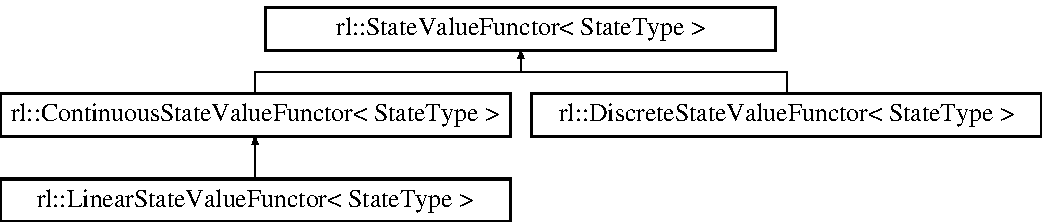
\includegraphics[height=2.978723cm]{structrl_1_1_state_value_functor}
\end{center}
\end{figure}
\subsection*{Public Member Functions}
\begin{DoxyCompactItemize}
\item 
\hypertarget{structrl_1_1_state_value_functor_a99a5f669d5f15febec82b4f7bfa840dc}{}\label{structrl_1_1_state_value_functor_a99a5f669d5f15febec82b4f7bfa840dc} 
virtual double {\bfseries operator()} (const State\+Type \&state) const =0
\end{DoxyCompactItemize}


\subsection{Detailed Description}
\subsubsection*{template$<$typename State\+Type$>$\newline
struct rl\+::\+State\+Value\+Functor$<$ State\+Type $>$}



Definition at line 49 of file state\+\_\+value\+\_\+functor.\+hpp.



The documentation for this struct was generated from the following file\+:\begin{DoxyCompactItemize}
\item 
/\+Users/davidfridovichkeil/\+Documents/\+Developer/rl/include/value/state\+\_\+value\+\_\+functor.\+hpp\end{DoxyCompactItemize}

\hypertarget{classrl_1_1_td_lambda}{}\section{rl\+:\+:Td\+Lambda$<$ State\+Type, Action\+Type $>$ Class Template Reference}
\label{classrl_1_1_td_lambda}\index{rl\+::\+Td\+Lambda$<$ State\+Type, Action\+Type $>$@{rl\+::\+Td\+Lambda$<$ State\+Type, Action\+Type $>$}}
\subsection*{Public Member Functions}
\begin{DoxyCompactItemize}
\item 
\hypertarget{classrl_1_1_td_lambda_a86d18da90b32c89f19b2e7eadcb4c5e4}{}\label{classrl_1_1_td_lambda_a86d18da90b32c89f19b2e7eadcb4c5e4} 
{\bfseries Td\+Lambda} (const State\+Type \&initial\+\_\+state, const \hyperlink{structrl_1_1_td_lambda_params}{Td\+Lambda\+Params} \&params)
\item 
\hypertarget{classrl_1_1_td_lambda_ab8eec2b22d9995865a22df9652dc35f3}{}\label{classrl_1_1_td_lambda_ab8eec2b22d9995865a22df9652dc35f3} 
bool {\bfseries Solve} (const \hyperlink{classrl_1_1_discrete_environment}{Discrete\+Environment}$<$ State\+Type, Action\+Type $>$ \&environment)
\item 
\hypertarget{classrl_1_1_td_lambda_aa76044eb47c107864d6ce575cdde7e87}{}\label{classrl_1_1_td_lambda_aa76044eb47c107864d6ce575cdde7e87} 
const \hyperlink{classrl_1_1_discrete_epsilon_greedy_policy}{Discrete\+Epsilon\+Greedy\+Policy}$<$ State\+Type, Action\+Type $>$ \& {\bfseries Policy} () const
\item 
\hypertarget{classrl_1_1_td_lambda_a411b370a455d6a6c145a2eb11f5b21fd}{}\label{classrl_1_1_td_lambda_a411b370a455d6a6c145a2eb11f5b21fd} 
const \hyperlink{structrl_1_1_discrete_state_value_functor}{Discrete\+State\+Value\+Functor}$<$ State\+Type $>$ \& {\bfseries Value} () const
\end{DoxyCompactItemize}


\subsection{Detailed Description}
\subsubsection*{template$<$typename State\+Type, typename Action\+Type$>$\newline
class rl\+::\+Td\+Lambda$<$ State\+Type, Action\+Type $>$}



Definition at line 57 of file td\+\_\+lambda.\+hpp.



The documentation for this class was generated from the following file\+:\begin{DoxyCompactItemize}
\item 
/\+Users/davidfridovichkeil/\+Documents/\+Developer/rl/include/solver/td\+\_\+lambda.\+hpp\end{DoxyCompactItemize}

\hypertarget{structrl_1_1_td_lambda_params}{}\section{rl\+:\+:Td\+Lambda\+Params Struct Reference}
\label{structrl_1_1_td_lambda_params}\index{rl\+::\+Td\+Lambda\+Params@{rl\+::\+Td\+Lambda\+Params}}
\subsection*{Public Attributes}
\begin{DoxyCompactItemize}
\item 
\hypertarget{structrl_1_1_td_lambda_params_ad5fcee919295c90b2a703e938869a709}{}\label{structrl_1_1_td_lambda_params_ad5fcee919295c90b2a703e938869a709} 
double {\bfseries discount\+\_\+factor\+\_\+} = 0.\+9
\item 
\hypertarget{structrl_1_1_td_lambda_params_aac69c9c13f56e139a88282ebcb9c1d2b}{}\label{structrl_1_1_td_lambda_params_aac69c9c13f56e139a88282ebcb9c1d2b} 
double {\bfseries lambda\+\_\+} = 0.\+5
\item 
\hypertarget{structrl_1_1_td_lambda_params_a40c12a22c1fbbc8891bb9530b5abf511}{}\label{structrl_1_1_td_lambda_params_a40c12a22c1fbbc8891bb9530b5abf511} 
double {\bfseries alpha\+\_\+} = 0.\+5
\item 
\hypertarget{structrl_1_1_td_lambda_params_a9dd04e2caf114f91f18c5f63793d547f}{}\label{structrl_1_1_td_lambda_params_a9dd04e2caf114f91f18c5f63793d547f} 
size\+\_\+t {\bfseries max\+\_\+iterations\+\_\+} = 100
\item 
\hypertarget{structrl_1_1_td_lambda_params_aa0168143470bf2dc81a52c59b103643a}{}\label{structrl_1_1_td_lambda_params_aa0168143470bf2dc81a52c59b103643a} 
size\+\_\+t {\bfseries num\+\_\+rollouts\+\_\+} = 1
\item 
\hypertarget{structrl_1_1_td_lambda_params_af1b8ab6c28edb093672fd6799675c3f4}{}\label{structrl_1_1_td_lambda_params_af1b8ab6c28edb093672fd6799675c3f4} 
int {\bfseries rollout\+\_\+length\+\_\+} = -\/1
\item 
\hypertarget{structrl_1_1_td_lambda_params_a11c7b952f11629bb5f18dd52648a4277}{}\label{structrl_1_1_td_lambda_params_a11c7b952f11629bb5f18dd52648a4277} 
double {\bfseries initial\+\_\+epsilon\+\_\+} = 0.\+5
\end{DoxyCompactItemize}


\subsection{Detailed Description}


Definition at line 48 of file td\+\_\+lambda\+\_\+params.\+hpp.



The documentation for this struct was generated from the following file\+:\begin{DoxyCompactItemize}
\item 
/\+Users/davidfridovichkeil/\+Documents/\+Developer/rl/include/solver/td\+\_\+lambda\+\_\+params.\+hpp\end{DoxyCompactItemize}

%--- End generated contents ---

% Index
\backmatter
\newpage
\phantomsection
\clearemptydoublepage
\addcontentsline{toc}{chapter}{Index}
\printindex

\end{document}
